\hfill \newline
\textbf{Analysis\#1} \newline
\phantom{ } We first built three circuits with the same schematic shown in figure[\ref{fig:circ1}] with the power supply $\pm12\si{\volt}$ to the amplifier but of different capacitors, where $R_1=R_2=240\si{\kilo\ohm},R_3=R_4=2.4\si{\kilo\ohm}$, and the left-to-right resistance of $R_5$ is $100\si{\kilo\ohm}$. According to the prelab result, we had the following values for capacitors, shown in table[\ref{tab:chos}].

\begin{figure}[!htbp]
	\centering
	\begin{framed}
		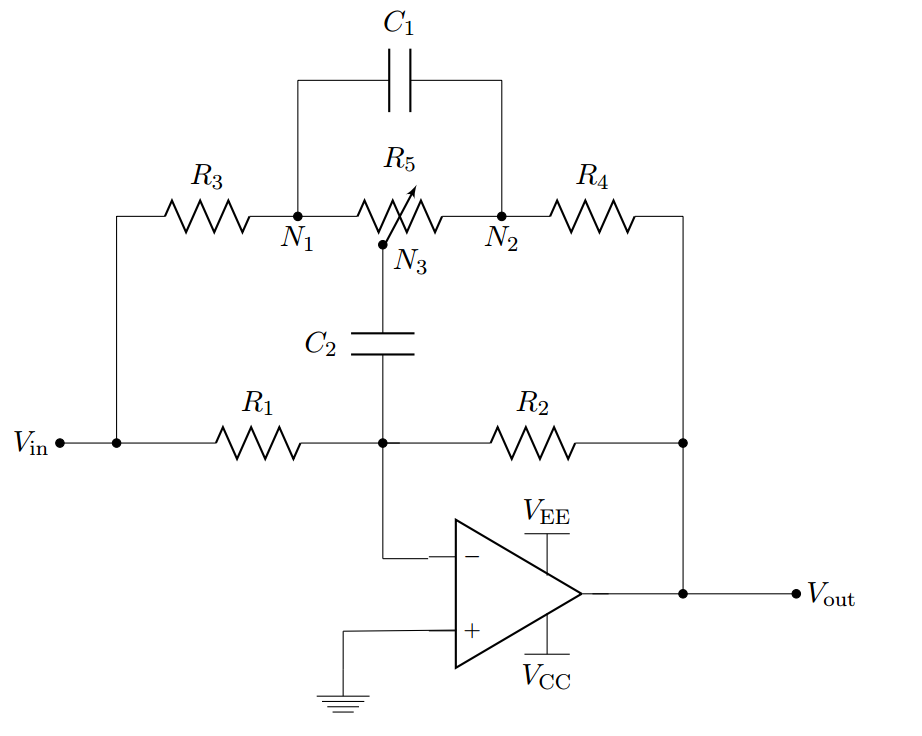
\includegraphics[width=\linewidth]{images/circ1.png}
		\caption{The equalizer filter schematic}
		\label{fig:circ1}
	\end{framed}
\end{figure}

\begin{table}[!htbp]
	\centering
	\caption{Capacitance of capacitors in the filters}
	\begin{tabular}{lcc}
		\toprule
		center frequency & $C_1$ & $C_2$ \\
		\midrule
		$250\si{\hertz}$ & $0.1\si{\micro\farad}$ & $0.0047\si{\micro\farad}$ \\
		$1\si{\kilo\hertz}$ & $0.022\si{\micro\farad}$ & $0.0022\si{\micro\farad}$ \\
		$4\si{\kilo\hertz}$ & $0.0056\si{\micro\farad}$ & $560\si{\pico\farad}$ \\
		\bottomrule
	\end{tabular}
	\label{tab:chos}
\end{table}

To make sure that those circuits works well as band-pass. We measured the frequency response of the gain of each circuit, in the 1-2-5 method, from $10\si{\hertz}$ to $5\si{\kilo\hertz}$. The results are displayed in table[\ref{tab:data00},\ref{tab:data01},\ref{tab:data02},\ref{tab:data10},\ref{tab:data11},\ref{tab:data12},\ref{tab:data20},\ref{tab:data21},\ref{tab:data22}].

\begin{table}[!htbp]
	\centering
	\caption{Measurements of $25\%$ - $250\si{\hertz}$}
	\label{tab:data00}
	\begin{tabular}{lccc}
		\toprule
		frequency($\si{\hertz}$) & $V_{in}$($\si{\milli\volt}$) & $V_{out}$($\si{\milli\volt}$) & gain($\si{\decibel}$) \\
		\midrule
		10	&224&	232&	0.305\\
		20	&232&	236&	0.148\\
		50	&232&	252&	0.718\\
		100	&224&	280&	1.938\\
		200	&220&	356&	4.181\\
		500	&220&	368&	4.469\\
		1000&	244&	280&	1.195\\
		2000&	232&	248&	0.579\\
		5000&	232&	244&	0.438\\
		10000&	232&	240&	0.294\\
		20000&	240&	224&	-0.599\\
		50000&	232&	228&	-0.151\\
		\bottomrule
	\end{tabular}
\end{table}

\begin{table}[!htbp]
	\centering
	\caption{Measurements of $25\%$ - $1\si{\kilo\hertz}$}
	\label{tab:data01}
	\begin{tabular}{lccc}
		\toprule
		frequency($\si{\hertz}$) & $V_{in}$($\si{\milli\volt}$) & $V_{out}$($\si{\milli\volt}$) & gain($\si{\decibel}$) \\
		\midrule
		10&	224&	232&	0.305\\
		20&	228&	228&	0.000\\
		50&	220&	224&	0.157\\
		100&	224&	236&	0.453\\
		200&	220&	268&	1.714\\
		500&	220&	384&	4.838\\
		1000&	224&	428&	5.624\\
		2000&	228&	324&	3.052\\
		5000&	228&	246&	0.660\\
		10000&	232&	232&	0.000\\
		20000&	236&	236&	0.000\\
		50000&	232&	240&	0.294\\
		\bottomrule
	\end{tabular}
\end{table}

\begin{table}[!htbp]
	\centering
	\caption{Measurements of $25\%$ - $4\si{\kilo\hertz}$}
	\label{tab:data02}
	\begin{tabular}{lccc}
		\toprule
		frequency($\si{\hertz}$) & $V_{in}$($\si{\milli\volt}$) & $V_{out}$($\si{\milli\volt}$) & gain($\si{\decibel}$) \\
		\midrule
		10&	220&	228&	0.310\\
		20&	224&	224&	0.000\\
		50&	224&	228&	0.154\\
		100&	220&	232&	0.461\\
		200&	224&	240&	0.599\\
		500&	224&	244&	0.743\\
		1000&	228&	280&	1.784\\
		2000&	228&	356&	3.870\\
		5000&	228&	392&	4.707\\
		10000&	228&	232&	0.151\\
		20000&	228&	228&	0.000\\
		50000&	228&	224&	-0.154\\
		\bottomrule
	\end{tabular}
\end{table}


\begin{table}[!htbp]
	\centering
	\caption{Measurements of $50\%$ - $250\si{\hertz}$}
	\label{tab:data10}
	\begin{tabular}{lccc}
		\toprule
		frequency($\si{\hertz}$) & $V_{in}$($\si{\milli\volt}$) & $V_{out}$($\si{\milli\volt}$) & gain($\si{\decibel}$) \\
		\midrule
		10&	228&	232&	0.151\\
		20&	220&	232&	0.461\\
		50&	220&	232&	0.461\\
		100&	236&	232&	-0.148\\
		200&	232&	232&	0.000\\
		500&	220&	232&	0.461\\
		1000&	236&	240&	0.146\\
		2000&	226&	240&	0.522\\
		5000&	232&	236&	0.148\\
		10000&	232&	208&	-0.948\\
		20000&	244&	192&	-2.082\\
		50000&	240&	192&	-1.938\\
		\bottomrule
	\end{tabular}
\end{table}

\begin{table}[!htbp]
	\centering
	\caption{Measurements of $50\%$ - $1\si{\kilo\hertz}$}
	\label{tab:data11}
	\begin{tabular}{lccc}
		\toprule
		frequency($\si{\hertz}$) & $V_{in}$($\si{\milli\volt}$) & $V_{out}$($\si{\milli\volt}$) & gain($\si{\decibel}$) \\
		\midrule
		10&	220&	232&	0.461\\
		20&	236&	232&	-0.148\\
		50&	232&	228&	-0.151\\
		100&	228&	232&	0.151\\
		200&	224&	228&	0.154\\
		500&	232&	244&	0.438\\
		1000&	220&	232&	0.461\\
		2000&	220&	236&	0.610\\
		5000&	224&	236&	0.453\\
		10000&	232&	204&	-1.117\\
		20000&	240&	216&	-0.915\\
		50000&	232&	196&	-1.465\\
		\bottomrule
	\end{tabular}
\end{table}

\begin{table}[!htbp]
	\centering
	\caption{Measurements of $50\%$ - $4\si{\kilo\hertz}$}
	\label{tab:data12}
	\begin{tabular}{lccc}
		\toprule
		frequency($\si{\hertz}$) & $V_{in}$($\si{\milli\volt}$) & $V_{out}$($\si{\milli\volt}$) & gain($\si{\decibel}$) \\
		\midrule
		10&	220&	240&	0.756\\
		20&	240&	228&	-0.446\\
		50&	228&	224&	-0.154\\
		100&	224&	228&	0.154\\
		200&	232&	236&	0.148\\
		500&	220&	240&	0.756\\
		1000&	232&	236&	0.148\\
		2000&	248&	252&	0.139\\
		5000&	232&	240&	0.294\\
		10000&	228&	192&	-1.493\\
		20000&	244&	220&	-0.899\\
		50000&	248&	200&	-1.868\\
		\bottomrule
	\end{tabular}
\end{table}


\begin{table}[!htbp]
	\centering
	\caption{Measurements of $75\%$ - $250\si{\hertz}$}
	\label{tab:data20}
	\begin{tabular}{lccc}
		\toprule
		frequency($\si{\hertz}$) & $V_{in}$($\si{\milli\volt}$) & $V_{out}$($\si{\milli\volt}$) & gain($\si{\decibel}$) \\
		\midrule
		10&	228&	224&	-0.154\\
		20&	220&	228&	0.310\\
		50&	220&	224&	0.157\\
		100&	220&	192&	-1.182\\
		200&	220&	160&	-2.766\\
		500&	224&	164&	-2.708\\
		1000&	240&	200&	-1.584\\
		2000&	224&	224&	0.000\\
		5000&	248&	228&	-0.730\\
		10000&	236&	192&	-1.792\\
		20000&	232&	216&	-0.621\\
		50000&	232&	224&	-0.305\\
		
		\bottomrule
	\end{tabular}
\end{table}

\begin{table}[!htbp]
	\centering
	\caption{Measurements of $75\%$ - $1\si{\kilo\hertz}$}
	\label{tab:data21}
	\begin{tabular}{lccc}
		\toprule
		frequency($\si{\hertz}$) & $V_{in}$($\si{\milli\volt}$) & $V_{out}$($\si{\milli\volt}$) & gain($\si{\decibel}$) \\
		\midrule
		10&	232&	220&	-0.461\\
		20&	220&	208&	-0.487\\
		50&	232&	162&	-3.119\\
		100&	224&	134&	-4.463\\
		200&	236&	124&	-5.590\\
		500&	224&	120&	-5.421\\
		1000&	232&	120&	-5.726\\
		2000&	232&	132&	-4.898\\
		5000&	240&	224&	-0.599\\
		10000&	232&	228&	-0.151\\
		20000&	232&	228&	-0.151\\
		50000&	228&	228&	0.000\\
		\bottomrule
	\end{tabular}
\end{table}

\begin{table}[!htbp]
	\centering
	\caption{Measurements of $75\%$ - $4\si{\kilo\hertz}$}
	\label{tab:data22}
	\begin{tabular}{lccc}
		\toprule
		frequency($\si{\hertz}$) & $V_{in}$($\si{\milli\volt}$) & $V_{out}$($\si{\milli\volt}$) & gain($\si{\decibel}$) \\
		\midrule
		10&	244&	232&	-0.438\\
		20&	220&	212&	-0.322\\
		50&	232&	220&	-0.461\\
		100&	220&	204&	-0.656\\
		200&	220&	196&	-1.003\\
		500&	224&	196&	-1.160\\
		1000&	220&	170&	-2.239\\
		2000&	220&	152&	-3.212\\
		5000&	224&	154&	-3.255\\
		10000&	236&	188&	-1.975\\
		20000&	232&	212&	-0.783\\
		50000&	232&	228&	-0.151\\
		\bottomrule
	\end{tabular}
\end{table}

\hfill \newline
\textbf{Analysis\#2} \newline
\phantom{ } According to the gain we measured, we then drew the plots to show that those circuits did work as adjustable band-pass and band-stop. 
\subsection{Set the potentiometer to $25\%$}
For the potentiometer at $25\%$, the plots are figure[\ref{fig:plot00},\ref{fig:plot01},\ref{fig:plot02}]. Using the plots, we figured out those constants of the filter in table[\ref{tab:cnst0}]. We can say that the filter is a band-pass filter, and the capacitors and resistor we used were good choices to achieve this function.

\begin{table}[!htbp]
	\centering
	\caption{Constants of the filter with potentiometer at $25\%$}
	\label{tab:cnst0}
	\begin{tabular}{ccc}
		\toprule
		center frequency($\si{\hertz}$) & $3-\si{\decibel}$ frequency($\si{\hertz}$) & maximum gain($\si{\decibel}$) \\
		theoretical and actual & left and right & or minimum\\
		\midrule
		250 | NA & NA | NA & 0.4454\\
		1000 | NA & NA | NA & 0.5654\\
		4000 | NA & NA | NA & 0.7558\\
		\bottomrule
	\end{tabular}
\end{table}

\begin{figure}
	\centering
	\begin{framed}
		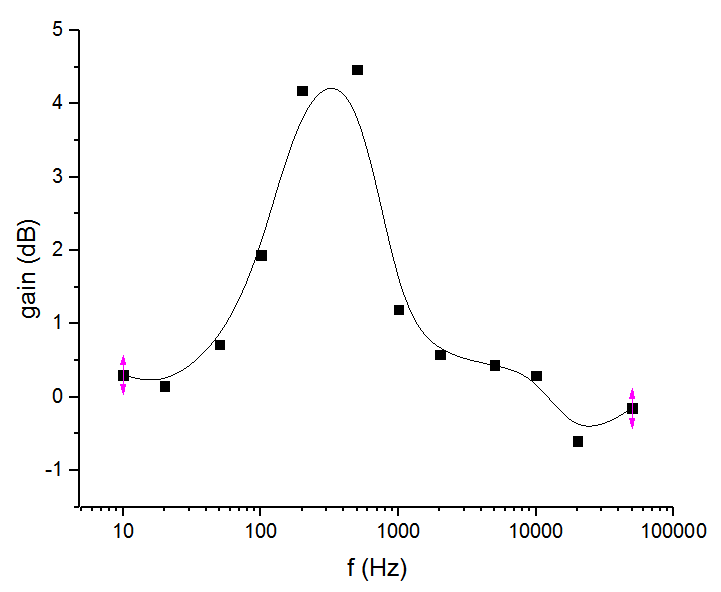
\includegraphics[width=\linewidth]{images/00.PNG}
		\caption{Plot of $25\%$ - $250\si{\hertz}$}
		\label{fig:plot00}
	\end{framed}
\end{figure}

\begin{figure}
	\centering
	\begin{framed}
		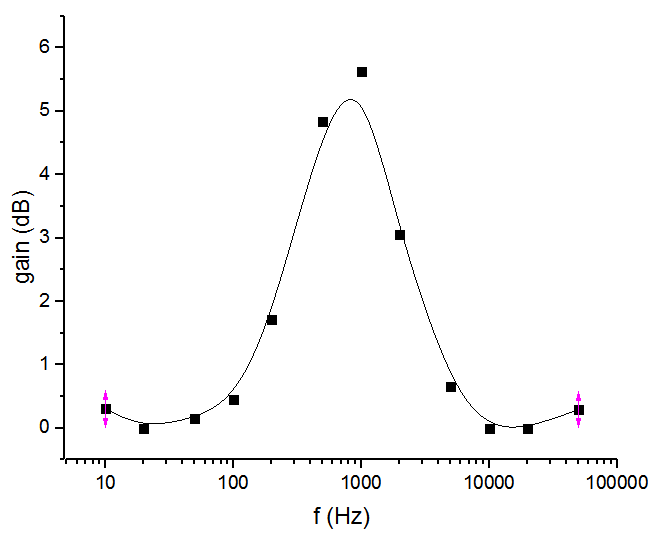
\includegraphics[width=\linewidth]{images/01.PNG}
		\caption{Plot of $25\%$ - $1\si{\kilo\hertz}$}
		\label{fig:plot01}
	\end{framed}
\end{figure}

\begin{figure}
	\centering
	\begin{framed}
		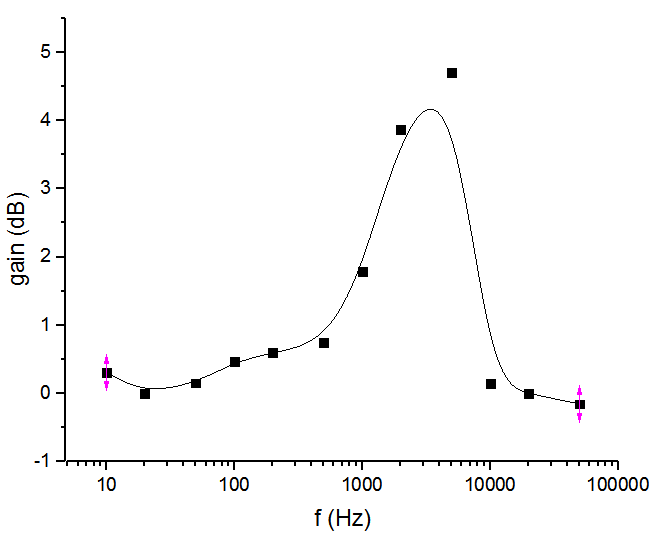
\includegraphics[width=\linewidth]{images/02.PNG}
		\caption{Plot of $25\%$ - $4\si{\kilo\hertz}$}
		\label{fig:plot02}
	\end{framed}
\end{figure}

\subsection{Set the potentiometer to $50\%$}
For the potentiometer at $50\%$, the plots are figure[\ref{fig:plot10},\ref{fig:plot11},\ref{fig:plot12}]. Using the plots, we figured out those constants of the filter in table[\ref{tab:cnst1}]. Notice that \textit{NA} takes the place of an unavailable figure. We can say that the circuits are neither band-passes nor band-stops. Moreover, it was hard to find their center frequencies.

\begin{table}[!htbp]
	\centering
	\caption{Constants of the filter with potentiometer at $50\%$}
	\label{tab:cnst1}
	\begin{tabular}{ccc}
		\toprule
		center frequency($\si{\hertz}$) & $3-\si{\decibel}$ frequency($\si{\hertz}$) & maximum gain($\si{\decibel}$) \\
		theoretical and actual & left and right & or minimum\\
		\midrule
		250 | 319.38 & 66.49 | 1162.04 & 4.235\\
		1000 | 822.60 & 221.04 | 2796.96 & 5.185\\
		4000 | 3411.79 & 663.79 | 9339.89 & 4.178\\
		\bottomrule
	\end{tabular}
\end{table}

\begin{figure}
	\centering
	\begin{framed}
		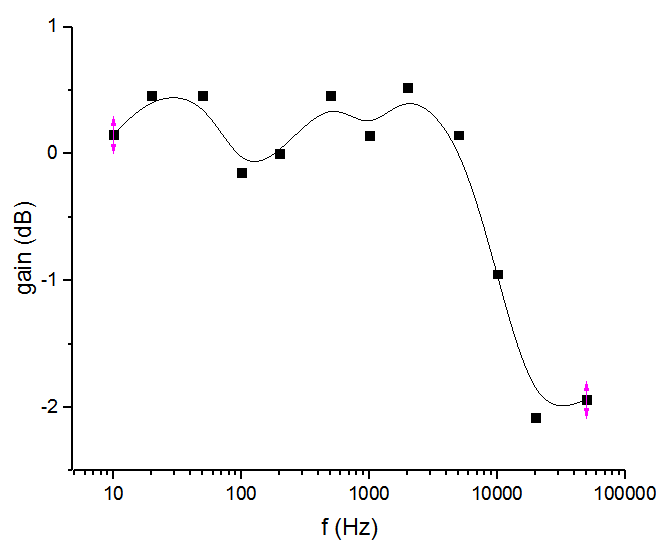
\includegraphics[width=\linewidth]{images/10.PNG}
		\caption{Plot of $50\%$ - $250\si{\hertz}$}
		\label{fig:plot10}
	\end{framed}
\end{figure}

\begin{figure}
	\centering
	\begin{framed}
		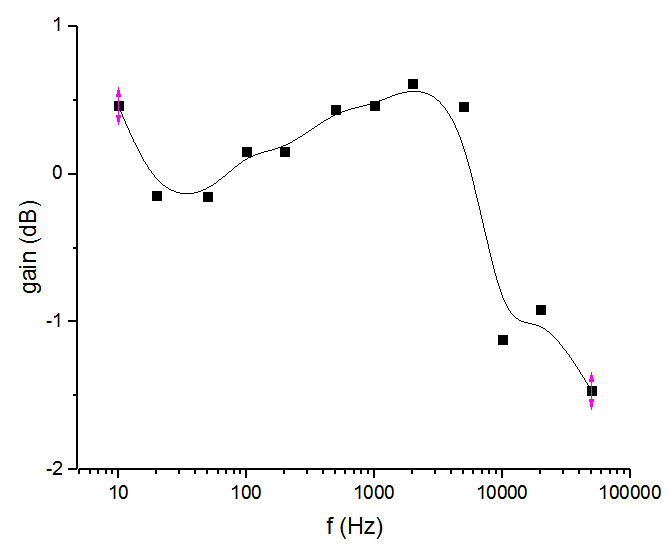
\includegraphics[width=\linewidth]{images/11.PNG}
		\caption{Plot of $50\%$ - $1\si{\kilo\hertz}$}
		\label{fig:plot11}
	\end{framed}
\end{figure}

\begin{figure}
	\centering
	\begin{framed}
		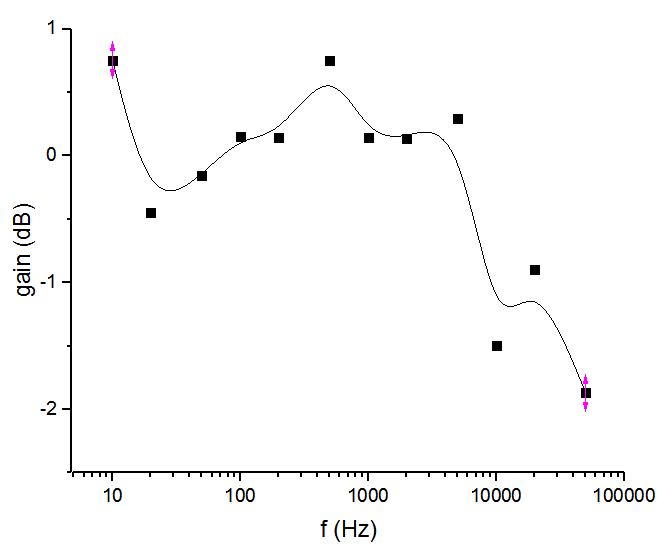
\includegraphics[width=\linewidth]{images/12.PNG}
		\caption{Plot of $50\%$ - $4\si{\kilo\hertz}$}
		\label{fig:plot12}
	\end{framed}
\end{figure}

\subsection{Set the potentiometer to $75\%$}
For the potentiometer at $75\%$, the plots are figure[\ref{fig:plot20},\ref{fig:plot21},\ref{fig:plot22}]. Using the plots, we figured out those constants of the filter in table[\ref{tab:cnst2}]. Notice that \textit{NA} represents not available and we actually used the minimum gain to describe the band-stop. We can say that the filter is a band-stop filter, proving again that the capacitors and resistor we used were good choices.

\begin{table}[!htbp]
	\centering
	\caption{Constants of the filter with potentiometer at $25\%$}
	\label{tab:cnst2}
	\begin{tabular}{ccc}
		\toprule
		center frequency($\si{\hertz}$) & $3-\si{\decibel}$ frequency($\si{\hertz}$) & maximum gain($\si{\decibel}$) \\
		theoretical and actual & left and right & or minimum\\
		\midrule
		250 | 311.54 & NA | NA & -2.685\\
		1000 | 868.40 & 43.00 | 3290.73 & -5.579\\
		4000 | 3173.96 & NA | NA & -3.196\\
		\bottomrule
	\end{tabular}
\end{table}

\begin{figure}
	\centering
	\begin{framed}
		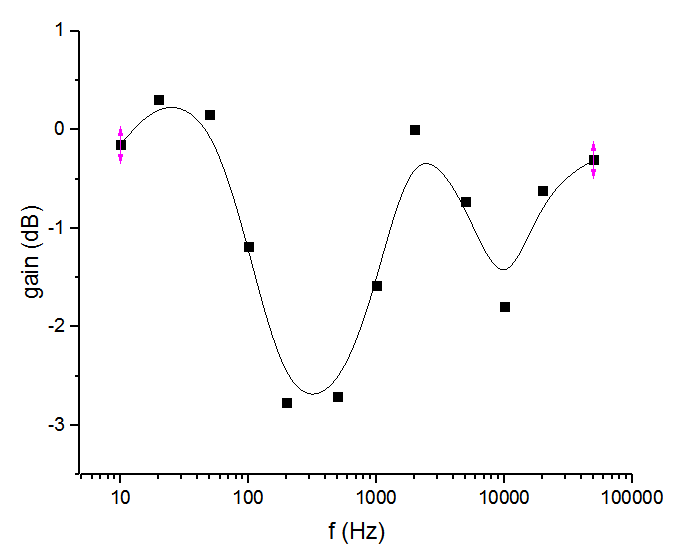
\includegraphics[width=\linewidth]{images/20.PNG}
		\caption{Plot of $75\%$ - $250\si{\hertz}$}
		\label{fig:plot20}
	\end{framed}
\end{figure}

\begin{figure}
	\centering
	\begin{framed}
		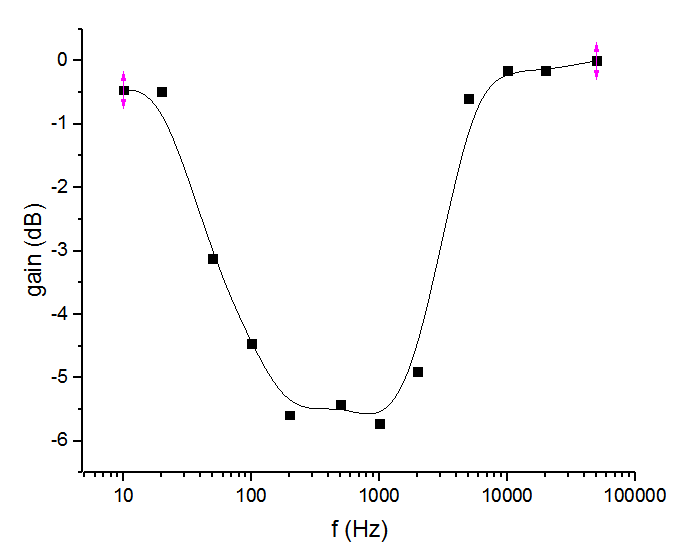
\includegraphics[width=\linewidth]{images/21.PNG}
		\caption{Plot of $75\%$ - $1\si{\kilo\hertz}$}
		\label{fig:plot21}
	\end{framed}
\end{figure}

\begin{figure}
	\centering
	\begin{framed}
		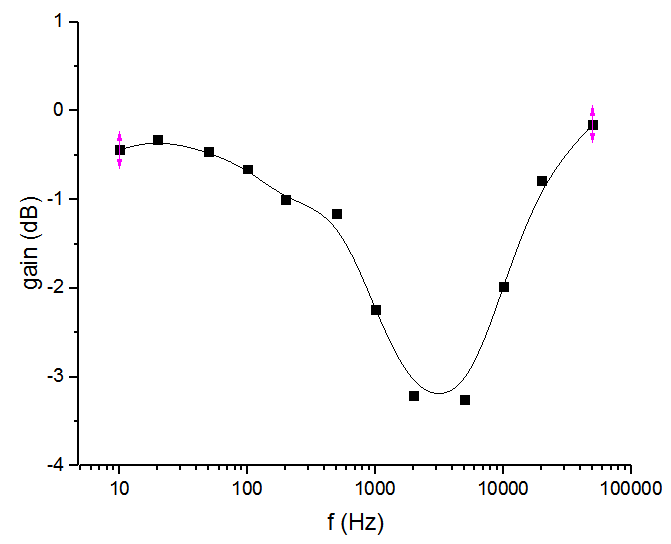
\includegraphics[width=\linewidth]{images/22.PNG}
		\caption{Plot of $75\%$ - $4\si{\kilo\hertz}$}
		\label{fig:plot22}
	\end{framed}
\end{figure}